\subsection{Comparación entre secuencial, vectorial y multicore}
Ya analizado el tipo de mejoras que son implementadas por GCC al utilizar -O1, -O2 y -O3, se presentan en esta sección los resultados de los experimentos realizados. Se comparan mediciones de tiempo de los distintos flags presentes en el compilador, con otras técnicas. 
~\\
~\\
En particular se estudian los flags -O0, -O1, -O2, -O3 y -Ofast para el compilador \textbf{GCC (GNU Compiler Collection)}, el compilador \textbf{ICC (Intel C++ Compiler)}, para \textbf{GCC+OpenMP (Open Multi-Processing)}, y por último -O0, -O3 y -Ofast para la versión vectorizada desarrollada en este trabajo, la cual consta de una parte en C++ en común con la versión no vectorial, que fue compilada con GCC, y una función implementada en Assembler y compilada mediante \textbf{NASM (Netwide Assembler x86)}, específicamente desarrollada para aprovechar la tecnología SIMD, y seleccionada por ser la sección más crítica en términos de rendimiento, del programa original.
~\\
~\\
Para cada técnica se experimentó con distintos tamaños del sistema simulado, comenzando desde simulaciones de sistemas pequeños de 1x1$m^2$ y aumentando de a un metro el lado del sistema, hasta llegar a 20x20$m^2$, el tamaño de lado es además la medida correspondiente al eje horizontal, mientras que el tiempo medido en segundos, es el correspondiente al eje vertical. En el caso en que se mide el efecto del tiempo del sistema simulado, se comienza con una duración de 1s y se llega aumentando de a 1s hasta 30s de sistema simulado. Además, para cada punto, se realizaron 100 repeticiones, y se tomó la medida y desvío estándar de las mismas, con el objetivo de eliminar el error de medición introducido por la falta de control del tiempo otorgado a las distintas tareas del sistema operativo por parte del scheduler. 
~\\
~\\
Todas las mediciones fueron realizadas mediante la utilización de la herramienta time de Linux, bajo la distribución Ubuntu 16.04 LTS, en una máquina \textbf{i7-920 2.67GHz, 18GB ram, 1TB HDD 7200rpm}. Además no se utilizó la máquina durante la experimentación, para no introducir ruido en las mediciones. En total se realizaron alrededor de \textbf{60.000 simulaciones}. A continuación se muestran los resultados de las mismas.
~\\
~\\

\begin{figure}[!htbp]
\caption{Tiempo(s) vs Tamaño(m) para GCC}
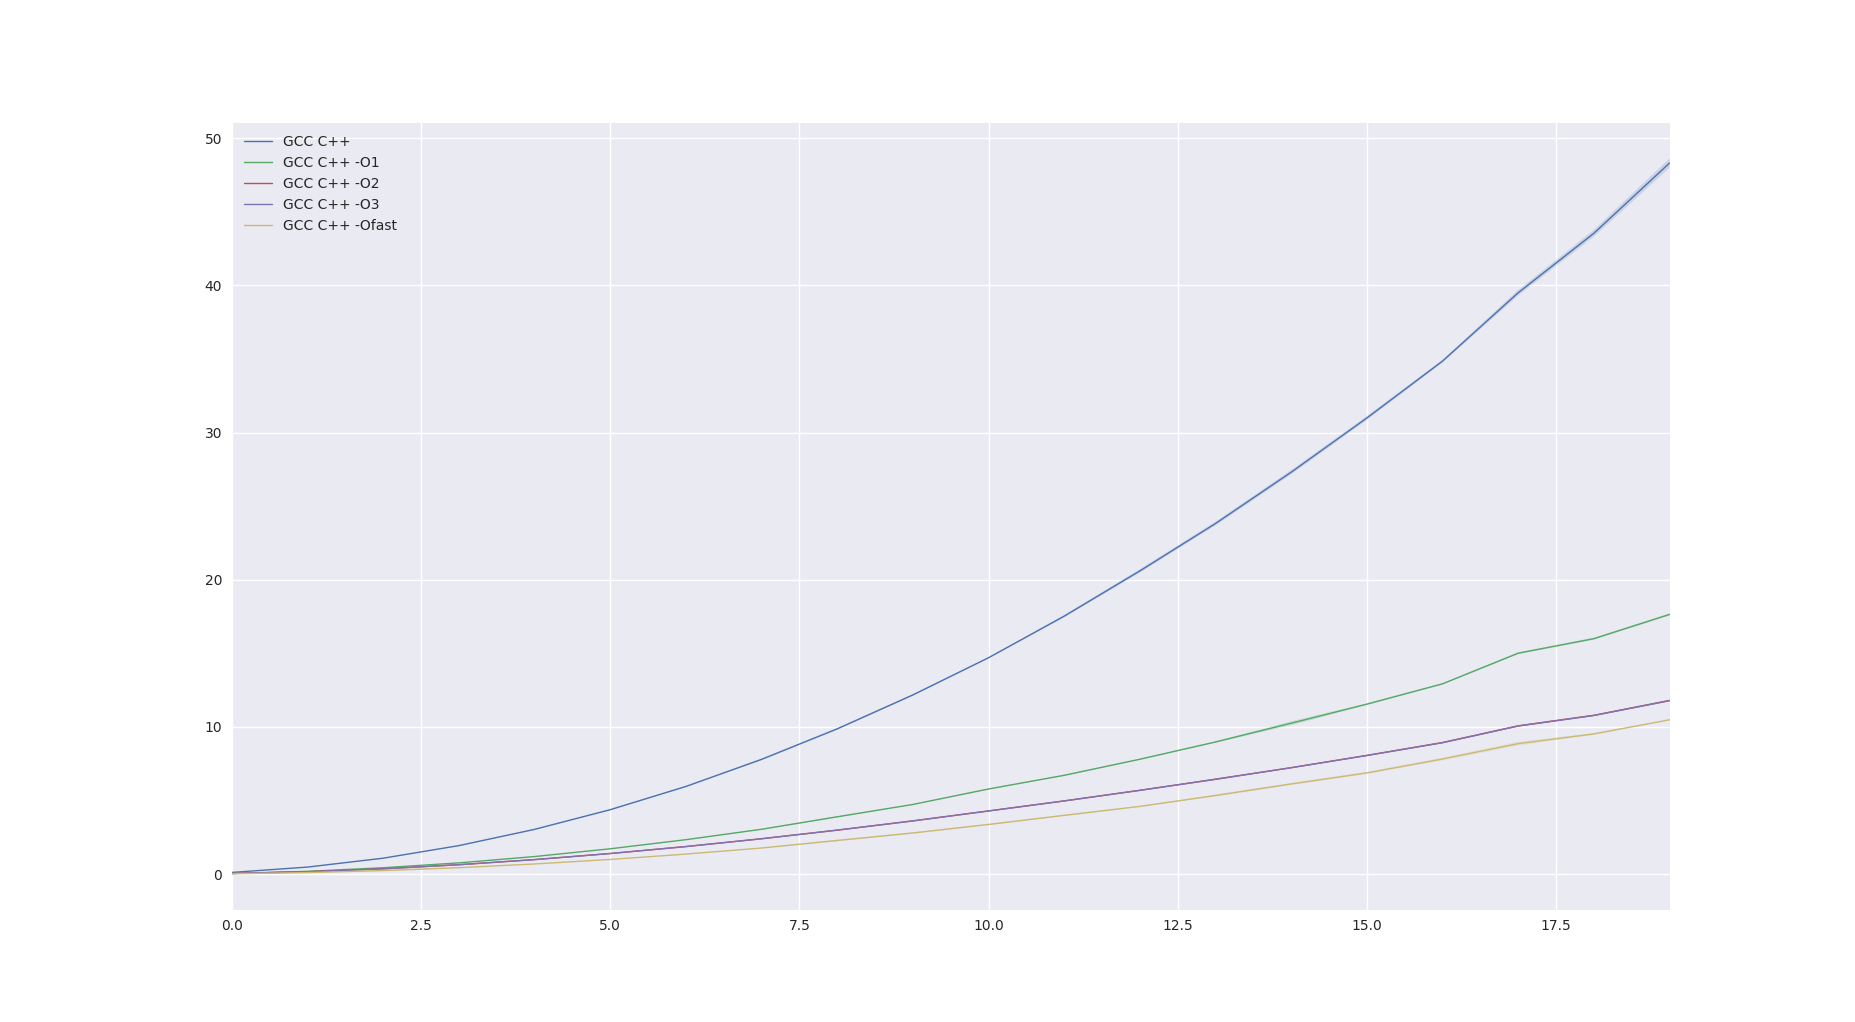
\includegraphics[width=\textwidth]{imagenes/plot_cpp.png}
\label{fig:plot_cpp}
\end{figure}

La primera experimentación consiste en el análisis de GCC, en particular su compilador C++, para distintos niveles de optimización. Esta se corresponde con la \textbf{Figura \ref{fig:plot_cpp}}.
~\\
~\\
Como es de esperar, el programa responde bien a las mejoras, con la mayor diferencia dándose entre -O0 y -O1, y la menor entre -O3 y -Ofast. Para el caso de mayor tamaño, el programa, distando de tardar casi 50s como en -O0, da un resultado menor a 20s, un tiempo menor a la mitad.
~\\
~\\
\begin{figure}[!htbp]
\caption{Tiempo(s) vs Tamaño(m) para Intel C++ Compiler}
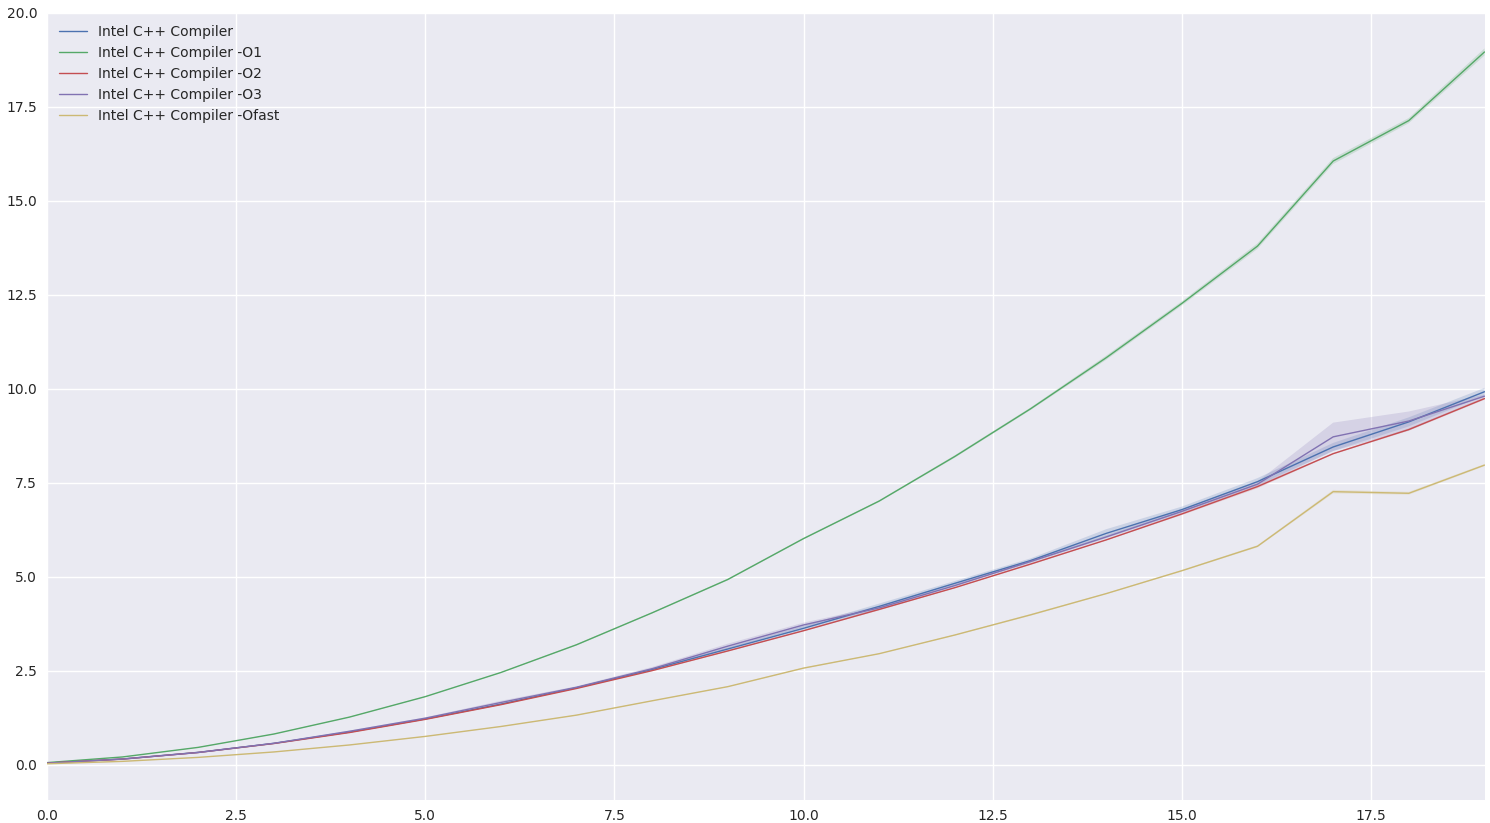
\includegraphics[width=\textwidth]{imagenes/plot_icc.png}
\label{fig:plot_icc}
\end{figure}

Donde la versión más optimizada de GCC daba un resultado para el tamaño de 20x20m, algo menor a 20s, el compilador ICC (Intel C++ compiler), muestra en la \textbf{Figura \ref{fig:plot_icc}} un tiempo de 10s, notablemente más rápido que  GCC -Ofast, sin utilizar optimizaciones. Esto se debe a que este compilador, como su nombre lo indica, fue diseñado para compilar para procesadores Intel, aprovechando las características específicas de los mismos. 
~\\
~\\
Se nota aquí otra diferencia, mientras que los flags llamados -Ox en GCC implementan siempre mejoras de velocidad de ejecución, el flag -O1, en ICC, busca mejorar el tamaño del ejecutable, dando así un tiempo de ejecución mayor que al no utilizar optimizaciones. Notar que aun así, este es más rápido que GCC -Ofast. Finalmente, la mejor medida para ICC esta alrededor de los 8s.
~\\
~\\
\begin{figure}[!htbp]
\caption{Tiempo(s) vs Tamaño(m) para Assembler(NASM)}
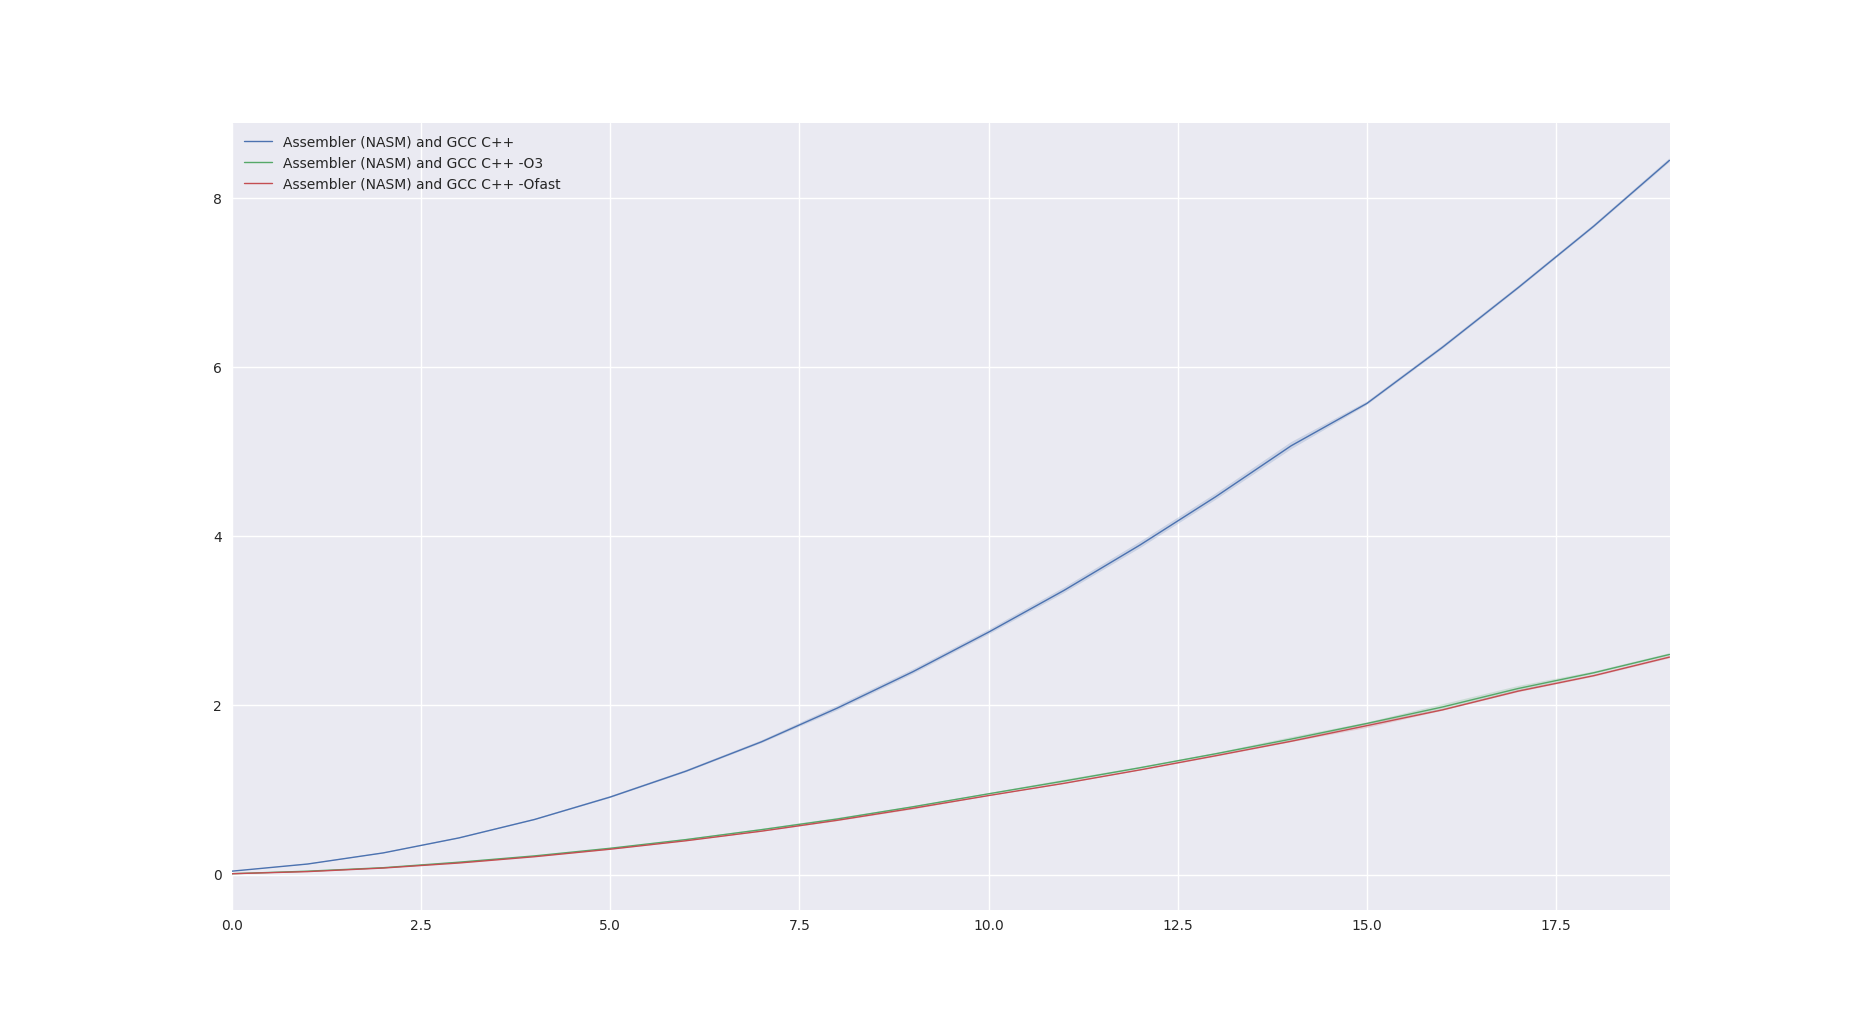
\includegraphics[width=\textwidth]{imagenes/plot_asm.png}
\label{fig:plot_asm}
\end{figure}

De la misma forma en que GCC -Ofast tenía un rendimiento similar a ICC sin optimizaciones, la versión producida en este trabajo, aprovechando la tecnología SIMD, tiene, sin optimizaciones, un rendimiento similar a ICC -Ofast. Esto puede verse en la \textbf{Figura \ref{fig:plot_asm}}. También muestra una mejora al utilizar flags, en particular llega a un tiempo de ejecución poco mayor a 2s, al utilizar -O3 u -Ofast, optimizaciones cuyas curvas son casi idénticas.
~\\
~\\
\begin{figure}[!htbp]
\caption{Tiempo(s) vs Tamaño(m) para GCC + OpenMP}
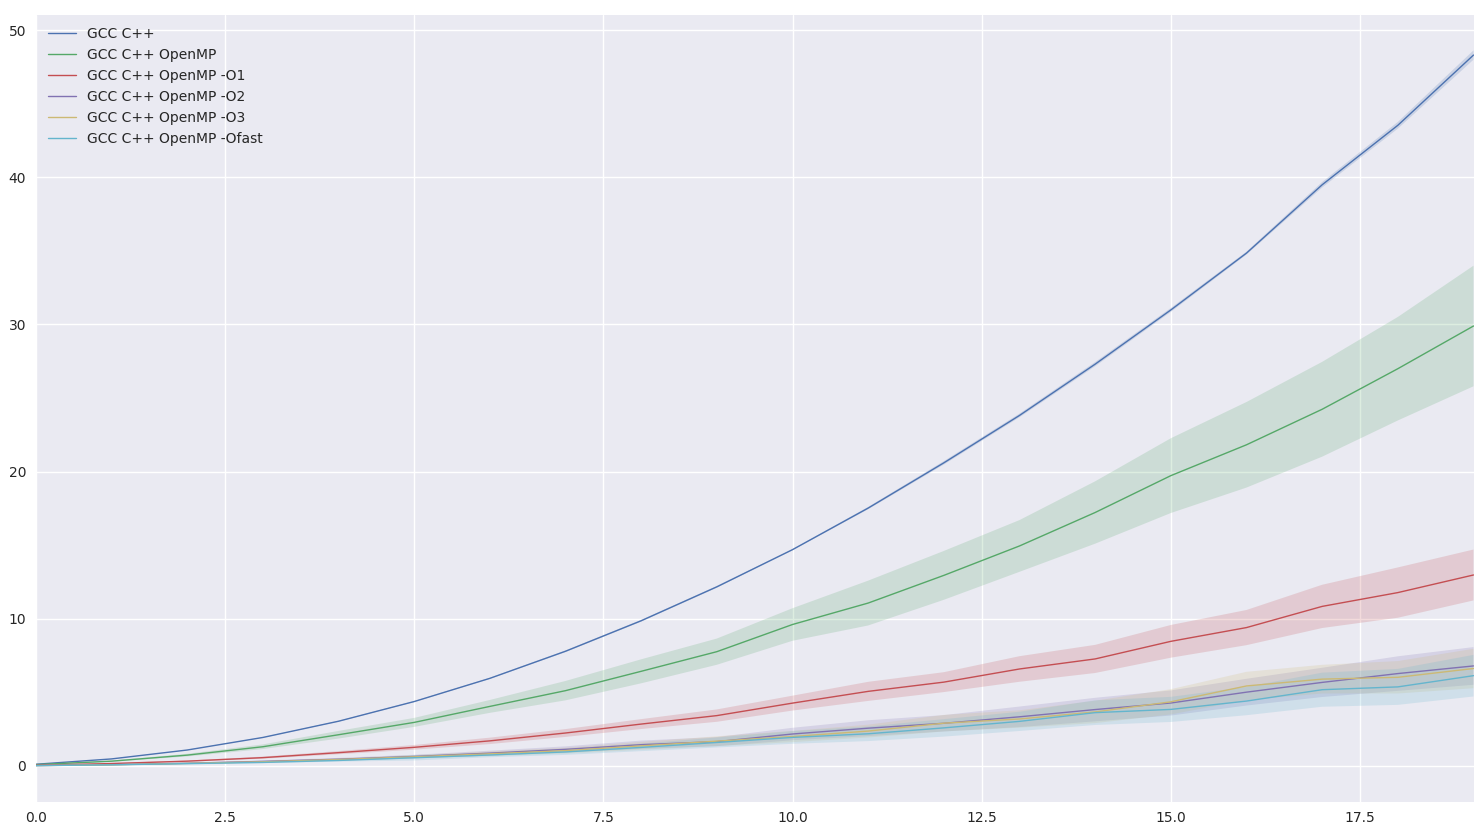
\includegraphics[width=\textwidth]{imagenes/plot_omp.png}
\label{fig:plot_omp}
\end{figure}
Otra experimentación surge de una estrategia distinta, en lugar de intentar mejorar el rendimiento mediante la optimización de código por si sola, se intentara hacer lo mismo mediante la asignación de mayor cantidad de recursos computacionales. OpenMP es una tecnología que logra hacer esto de forma automática. Se dispone, mediante el mismo, de directivas que al actuar sobre un ciclo que depende de una variable, ejecuta distintas instancias del cuerpo del mismo en distintos núcleos del procesador, logrando paralelización a nivel CPU, reduciendo los tiempos de ejecución.
~\\
~\\
Los resultados correspondientes a esta experimentación, pueden verse en la \textbf{Figura \ref{fig:plot_omp}}. Una particularidad de esta gráfica, es que muestra intervalos de desviación estándar mayores que las otras. Dado que estamos agregando recursos computacionales, el uso de CPU aumenta, dejando pocos recursos para atender al resto de las tareas del sistema operativo. Se sospecha que este es el principal motivo, para el aumento drástico de la varianza de las mediciones respecto de los otros experimentos.
~\\
~\\
Notamos que aunque la asignación de mayor cantidad de recursos aumenta significativamente el rendimiento, este no supera a la versión SIMD. Hay una explicación razonable para este fenómeno, la máquina donde se realizó la experimentación, como se comentó anteriormente, utiliza un i7-920 2.67GHz. Este modelo de procesador dispone de 4 núcleos físicos, con lo cual OpenMP puede gracias a esto, dividir la tarea en 4 partes. La versión SIMD del programa, utiliza registros XMM, y valores flotantes de 32 bits de longitud, con lo cual logra, mediante vectorización, procesar 4 puntos de la malla al mismo tiempo. Siendo que ambas técnicas procesan un máximo teórico de 4 puntos de malla por cada ejecución del cuerpo del ciclo, y que SIMD no requiere coordinación entre distintos núcleos, este resulta en mejores prestaciones.

\begin{figure}[!htbp]
\caption{Tiempo(s) vs Tamaño(m) utilizando el flag -Ofast}
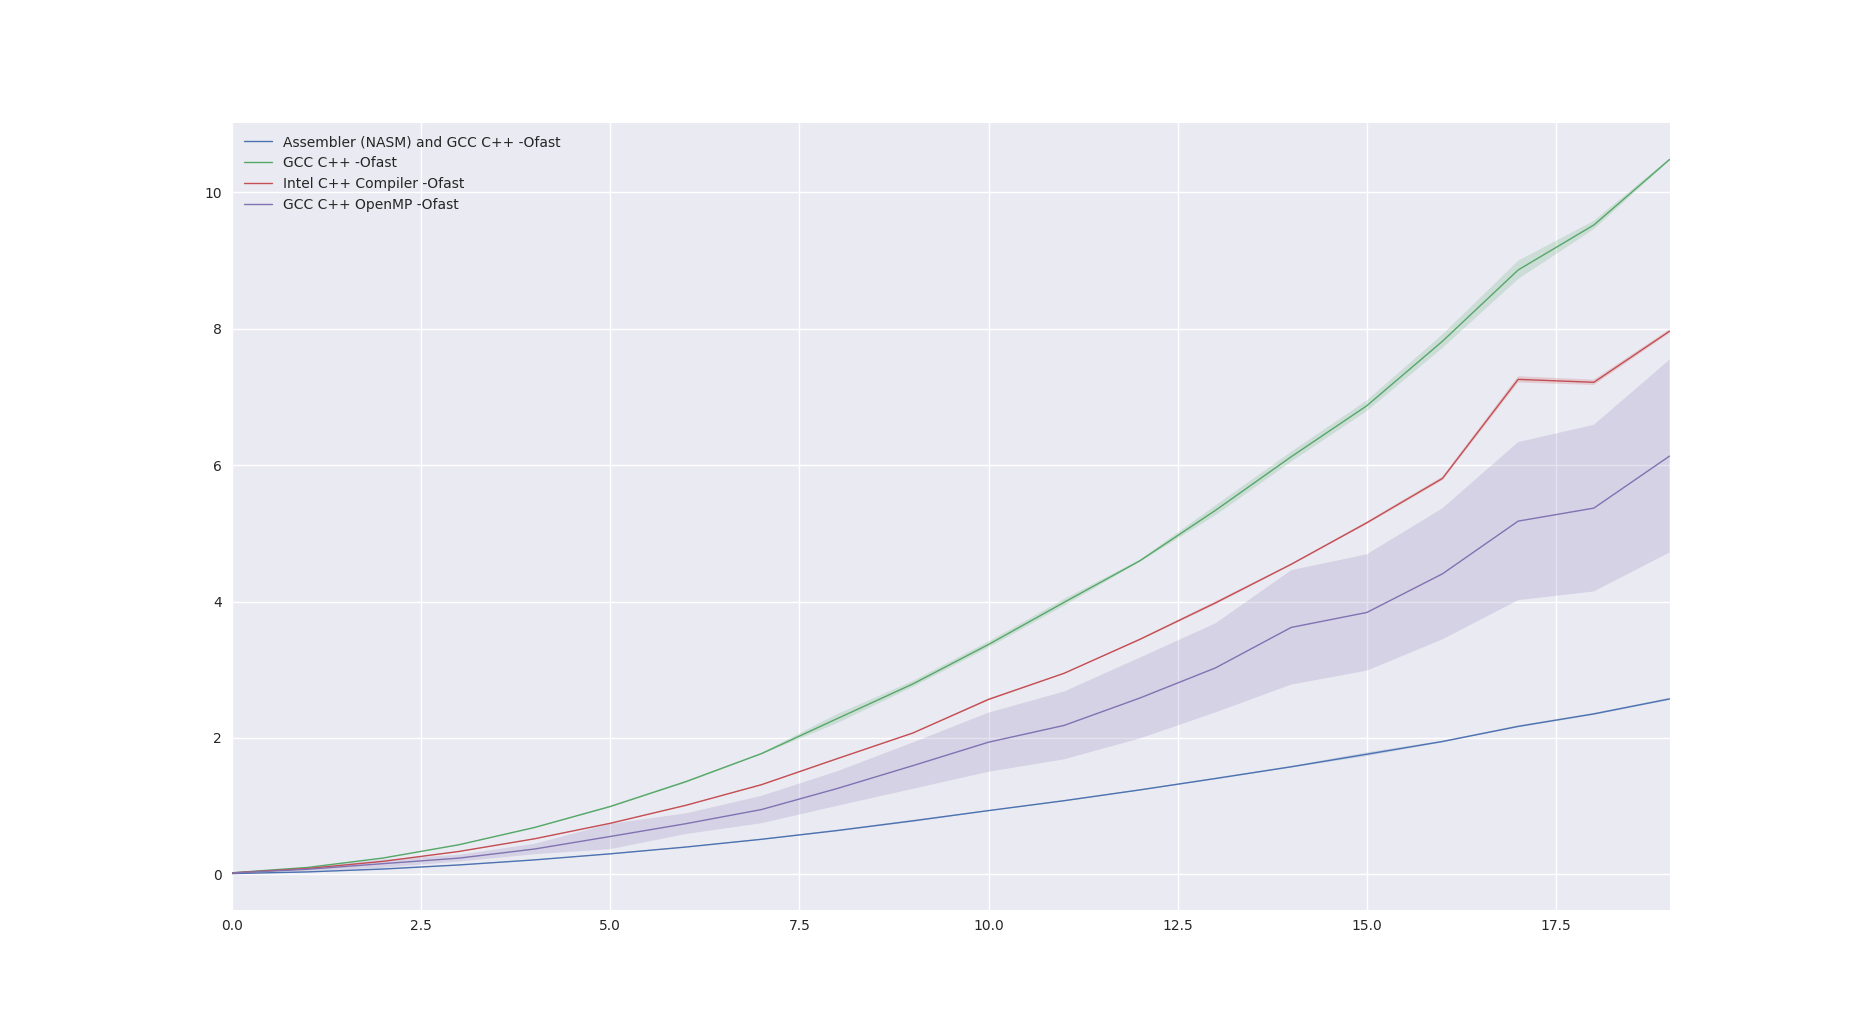
\includegraphics[width=\textwidth]{imagenes/plot_ofast.png}
\label{fig:plot_ofast}
\end{figure}
~\\
~\\

A modo ilustrativo, presentamos en la \textbf{Figura \ref{fig:plot_ofast}} una gráfica de las optimizaciones que dieron mejor resultado para cada técnica o compilador utilizado. En todos los casos el mejor rendimiento se obtuvo mediante la utilización del flag -Ofast. Queda claro mediante esta figura, que las mejores prestaciones se dan al utilizar SIMD, seguido por OpenMP, ICC, y finalmente GCC. El patrón queda claro, mientras más recursos se utilicen, y más específico sea el código de acuerdo a la plataforma subyacente, mejor rendimiento se obtiene. 



\begin{figure}[!htbp]
\caption{Tiempo real(s) vs Tiempo simulado(m) utilizando el flag -Ofast}
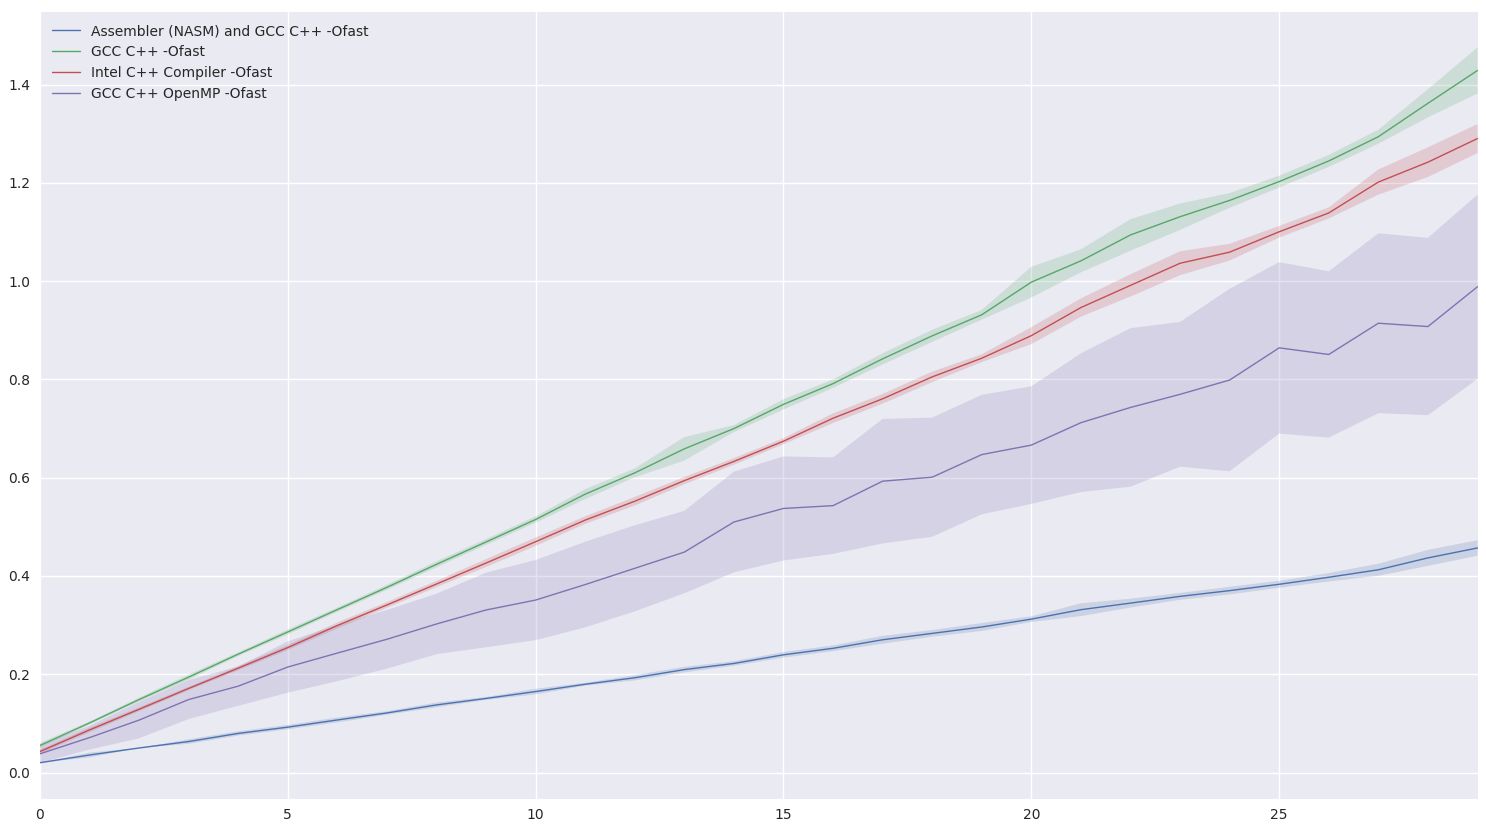
\includegraphics[width=\textwidth]{imagenes/plot_time_omp_unused.png}
\label{fig:plot_time_omp_unused}
\end{figure}

Finalmente se realiza un análisis de la única otra variable que afecta el rendimiento que es la magnitud de la cantidad de iteraciones temporales realizadas en cada simulación. En la \textbf{Figura \ref{fig:plot_time_omp_unused}} puede verse una comparación de los distintos casos analizados anteriormente, pero esta vez no aumenta el tamaño, aumenta el tiempo del sistema dinámico simulado. Cada punto de la gráfica indica un aumento del tiempo de un segundo más de simulación. 


\subsection{Análisis de performance bajo carga}


Por último se analiza el efecto del uso de CPU en otras tareas. Esto consta de ejecutar repetidamente simulaciones idénticas para los distintos casos que se analizan en este trabajo, medir el tiempo que tardan en terminar. Además a lo largo del experimento se lanzan dos tareas. La primera es una tarea que hace uso intensivo de accesos a memoria, y la segunda de operaciones de cálculo flotante, utilizando para esto la ALU (Arithmetic Logic Unit). La ejecución de estas tareas genera dos picos en las mediciones de  las simulaciones de fluidos. Los resultados pueden apreciarse en la \textbf{Figura \ref{fig:plot_stress_test_ram_cpu}}. 
\begin{figure}[!htbp]
\caption{Tiempo(s) con carga de Memoria y luego CPU}
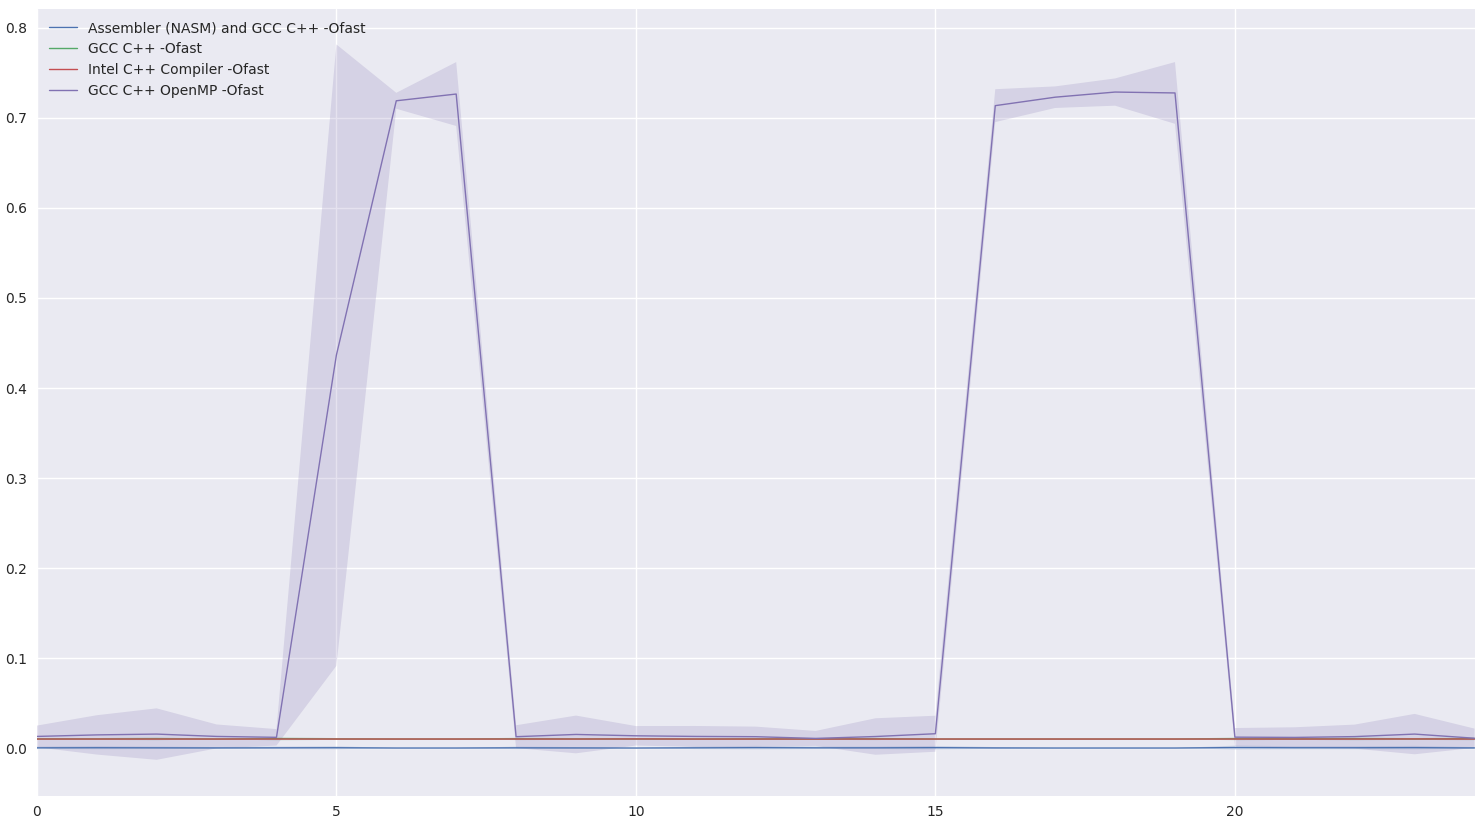
\includegraphics[width=\textwidth]{imagenes/plot_stress_test_ram_cpu.png}
\label{fig:plot_stress_test_ram_cpu}
\end{figure}
~\\
~\\
Podemos confirmar que la versión que utiliza OpenMP es la única que se ve afectada significativamente por la presencia de otras tareas, y también que no hay diferencias significativas entre tareas que usen memoria o tareas que realicen operaciones de punto flotante.




